\section{Search Based Test in Load, Performance and Stress Tests}

The search for the longest execution time is regarded as a discontinuous, nonlinear, optimization problem, with the input domain of the system under test as search space \cite{Sullivan}. The main objective of search based testing in performance,stress and load tests is to find test scenarios which produce execution times violating the timing constraints specified. If a temporal error is found, the test was successful \cite{Sullivan}. The application of evolutionary algorithms to load, performance and stress tests involves finding the best and worst case execution times (BCET, WCET) to determine if timing constraints are fulfilled \cite{Afzal2009a}. 

Some Search Based Tests uses a cost (fitnesse) function to select the best individuals. There has two measurement units normally associated with the fitnesse function in load, performance or stress test: Processor Cycles and Execution Time. The Processor Cycles approach describes a fitness function in terms of processor cycles. The Execution Time approach involves executing the application under test measuring the execution time \cite{Afzal2009} \cite{tracey2000search}.
% * <naubergois@gmail.com> 2015-09-17T01:17:52.488Z:
%
%  Rever esse paragrafo
%
The Table \ref{tab:comparison}  shows a comparison between the presented research work and the load, performance and stress test researches presented by Afzal et. al. \cite{Afzal2009}. Afzal's work was added with some of the latest research in the area (\cite{Garousi2006} \cite{Garousi2010} \cite{DiAlesio2013} \cite{DiAlesio2014} \cite{Alesio2015}). 


The columns represents the type of tool used ( Prototype or Functional Tool )  and the rows presents the metaheuristic used by each research (Genetic Algorithm, Tabu Search, Simulated Annnealing or a Customized Algorithm). The Table also divides the researches by the type of function fitnesse (Execution Time or Processor Cycles). Most research is limited to making prototypes on genetic algorithms. The presented research work is distinguished from others by having a functional tool using a hybrid approach. 



% * <naubergois@gmail.com> 2015-09-17T01:22:09.554Z:
%
%  Customized Algorithm
%

%\begin{figure}[h]
%\centering
%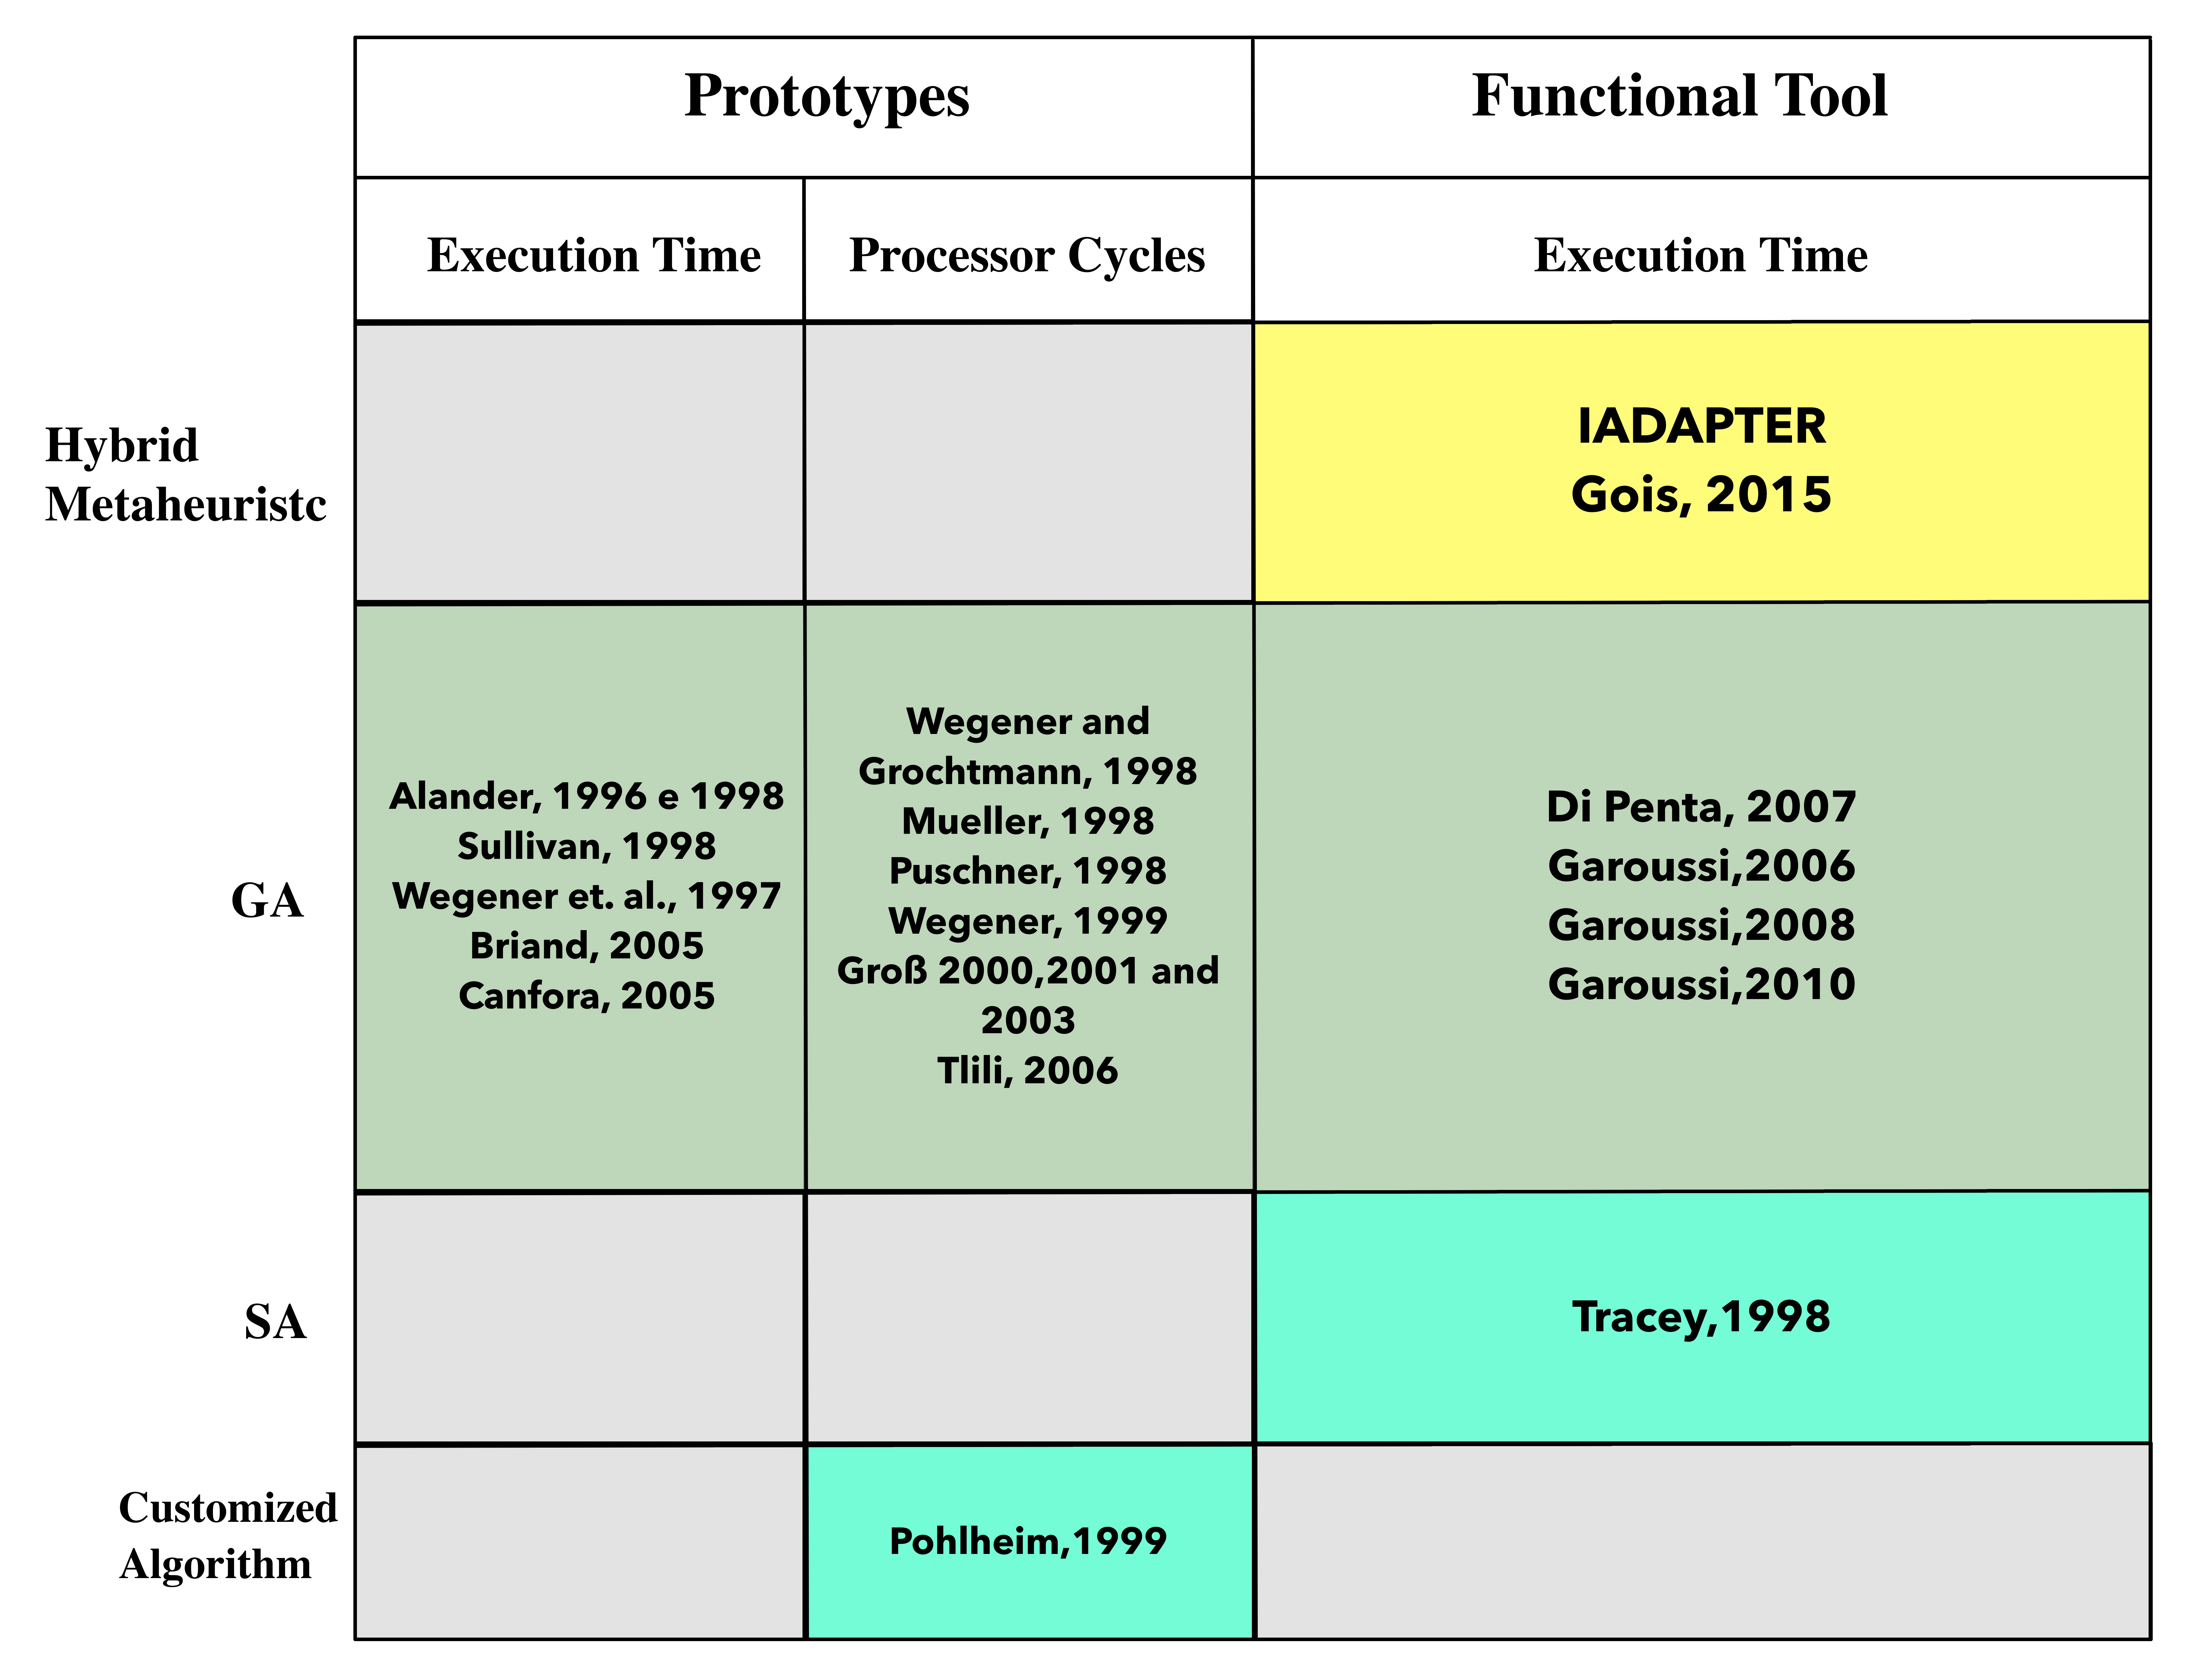
\includegraphics[width=0.5\textwidth]{./images/comparativo1.png}
%\caption{
%Distribution of the researches over range of applied metaheuristics}
%\label{fig:comparison}
%\end{figure}

% Please add the following required packages to your document preamble:
% \usepackage[table,xcdraw]{xcolor}
% If you use beamer only pass "xcolor=table" option, i.e. \documentclass[xcolor=table]{beamer}
\begin{table}[h]
\centering
\caption{Distribution of the researches over range of applied metaheuristics}
\label{tab:comparison}
\begin{tabular}{p{1.2cm}|p{1.8cm}|p{1.8cm}|p{1.8cm}|}
\cline{2-4}
                                                                & \multicolumn{2}{c|}{\textbf{Prototypes}}            & \textbf{Functional Tool} \\ \cline{2-4} 
                                                                & \begin{minipage}{0.2\textwidth}\footnotesize Execution Time  \end{minipage}          & \begin{minipage}{0.2\textwidth}\footnotesize Processor Cycles \end{minipage}        & \begin{minipage}{0.2\textwidth}\footnotesize Execution Time \end{minipage}           \\ \cline{2-4} 
%\setlength{\extrarowheight}{20pt}
\begin{tabular}[c]{@{}l@{}}\begin{minipage}{0.1\textwidth}\scriptsize GA + SA  \\ + Tabu \\ Search \end{minipage}\end{tabular}  & \cellcolor[HTML]{FFCCC9} & \cellcolor[HTML]{FFCCC9} & \cellcolor[HTML]{F8FF00} \begin{minipage}{0.2\textwidth} \scriptsize \textbf{  \\ IADAPTER \\ Gois, 2015 \\} \end{minipage}  \\[2ex] \cline{2-4} 
\begin{minipage}{0.1\textwidth}\scriptsize GA \end{minipage}                                                              & \cellcolor[HTML]{CD9934} \begin{minipage}{0.12\textwidth}   \tiny \textnormal{ \\  Alander et al.,1998 \cite{Alander} \\ Wegener et al., 1996 and 1997 \cite{Wegener1997}\cite{J.WegenerK.GrimmM.GrochtmannH.Sthamer1996} \\  Sullivan et al., 1998 \cite{Sullivan} \\ Briand et al., 2005 \cite{Briand2005} \\ Canfora et al., 2005 \cite{Canfora}  \\ }\end{minipage} & \cellcolor[HTML]{CD9934} \begin{minipage}{0.12\textwidth} \tiny \textrm{  \\ Wegener and Grochtmann, 1998 \cite{Wegener1998} \\  Mueller et al., 1998 \cite{Mueller1998} \\ Puschner et al. \cite{Puschner1998} \\ Wegener et al., 2000 \cite{Stations} \\ Gro et al., 2000 \cite{Gross2000}  \\ }\end{minipage}& \cellcolor[HTML]{CD9934} \begin{minipage}{0.12\textwidth}   \tiny \textnormal{ \\  Di Penta, 2007 \cite{Penta2007} \\ Garoussi, 2006 \cite{Garousi2006} \\ Garousi, 2008 \cite{Garousi2008} \\ Garousi, 2010 \cite{Garousi2010} \\ } \end{minipage} \\[2ex] \cline{2-4} 
\begin{minipage}{0.1\textwidth}\scriptsize Simulated \\ Annealing \\ (SA) \end{minipage}                                                             & \cellcolor[HTML]{FFCCC9} & \cellcolor[HTML]{FFCCC9} & \cellcolor[HTML]{CD9934} \begin{minipage}{0.12\textwidth}   \tiny  Tracey, 1998 \cite{Tracey1998} \end{minipage} \\[2ex] \cline{2-4}
\begin{minipage}{0.1\textwidth}\scriptsize  Constraint \\ Programming \end{minipage}                                                             & \cellcolor[HTML]{FFCCC9} & \cellcolor[HTML]{FFCCC9} & \cellcolor[HTML]{CD9934} \begin{minipage}{0.12\textwidth}   \tiny  Alesio, 2014 \cite{DiAlesio2014} \\ Alesio, 2013 \cite{DiAlesio2013}  \end{minipage} \\[2ex] \cline{2-4} 
\begin{minipage}{0.1\textwidth}\scriptsize  GA +\\ Constraint \\ Programming \end{minipage}                                                             & \cellcolor[HTML]{FFCCC9} & \cellcolor[HTML]{FFCCC9} & \cellcolor[HTML]{CD9934} \begin{minipage}{0.12\textwidth}   \tiny  Alesio, 2015 \cite{Alesio2015} \end{minipage} \\[2ex] \cline{2-4} 
\setlength{\extrarowheight}{20pt}
\begin{tabular}[c]{@{}l@{}}
\begin{minipage}{0.1\textwidth}\scriptsize Customized \\ Algorithm \end{minipage}\end{tabular} & \cellcolor[HTML]{FFCCC9} & \cellcolor[HTML]{CD9934}  \begin{minipage}{0.12\textwidth}   \tiny  \textnormal{   \raggedleft Pohlheim, 1999 \cite{Pohlheim2005}  } \end{minipage} & \cellcolor[HTML]{FFCCC9} \\[4ex] \cline{2-4}
\end{tabular}
%\begin{tabular}[c]{@{}l@{}}
%\begin{minipage}{0.1\textwidth}\scriptsize GA  Constraint Programming \end{minipage}\end{tabular} & \cellcolor[HTML]{FFCCC9} & \cellcolor[HTML]{CD9934}  \begin{minipage}{0.12\textwidth}   \tiny  \textnormal{   \raggedleft Alesio, 2015 \cite{Alesio2015}   } \end{minipage} & \cellcolor[HTML]{FFCCC9} \\[4ex] \cline{2-4}
%\end{tabular}
\end{table}


The presented research work and Alesio's approach \cite{Alesio2015} uses a hybrid approach with a functional tool. The table \ref{tab:alesiogois} presents the main differences between Alesio's and Gois's approaches. While the present research uses an approach based on usage scenarios performing tests on an application installed in an available environment, Alesio use sequence diagrams  to select for arrival time of tasks in Systems from  safety-critical domains. 

\begin{table}[h]
\centering
\caption{Main differences between Alesio's \cite{Alesio2015} and Gois's approaches}
\label{tab:alesiogois}
\begin{tabular}{l|l|l|}
\cline{2-3}
                                                                                  & Alesio et al. \cite{Alesio2015}                                                                                                             & Gois et al.                                                                                                                            \\ \hline
\multicolumn{1}{|l|}{Metaheuristcs}                                               & \begin{tabular}[c]{@{}l@{}}GA+ \\ Constraint Programming\end{tabular}                                                      & \begin{tabular}[c]{@{}l@{}}GA+SA+\\ Tabu Search\end{tabular}                                                                           \\ \hline
\multicolumn{1}{|l|}{Inputs}                                                      & \begin{tabular}[c]{@{}l@{}}Design Model (Time and \\ Concurrency\\  Information)\end{tabular}                              & \begin{tabular}[c]{@{}l@{}}Number of Users\\ Ramp-up\\ Test scenarios\end{tabular}                                                     \\ \hline
\multicolumn{1}{|l|}{\begin{tabular}[c]{@{}l@{}}Main\\ Objective\end{tabular}}    & \begin{tabular}[c]{@{}l@{}}Find task arrival times\\ of aperiodic tasks that\\  maximizing\\  deadline misses\end{tabular} & \begin{tabular}[c]{@{}l@{}}Find the number of\\  users, ramp-up and \\ test scenarios that\\ maximizing\\ deadline misses\end{tabular} \\ \hline
\multicolumn{1}{|l|}{\begin{tabular}[c]{@{}l@{}}Main \\ Application\end{tabular}} & \begin{tabular}[c]{@{}l@{}}Systems from \\ safety-critical \\ domains\end{tabular}                                         & \begin{tabular}[c]{@{}l@{}}Web and Mobile \\ applications\end{tabular}                                                                 \\ \hline
\end{tabular}
\end{table}



%\nocite{Alander,Sullivan,Wegener1997,Briand2005,Canfora,Wegener1998,Mueller1998,Puschner1998,Wegener1999,Gro,Gross2003,Tlili1917}